\documentclass{article}
\usepackage[margin=20mm]{geometry}
\usepackage{tikz}
\usetikzlibrary{arrows.meta,positioning}
\pagestyle{empty}
\begin{document}
\begin{center}
{\Large Round 3: Evidence-driven offline planning}\\[10mm]
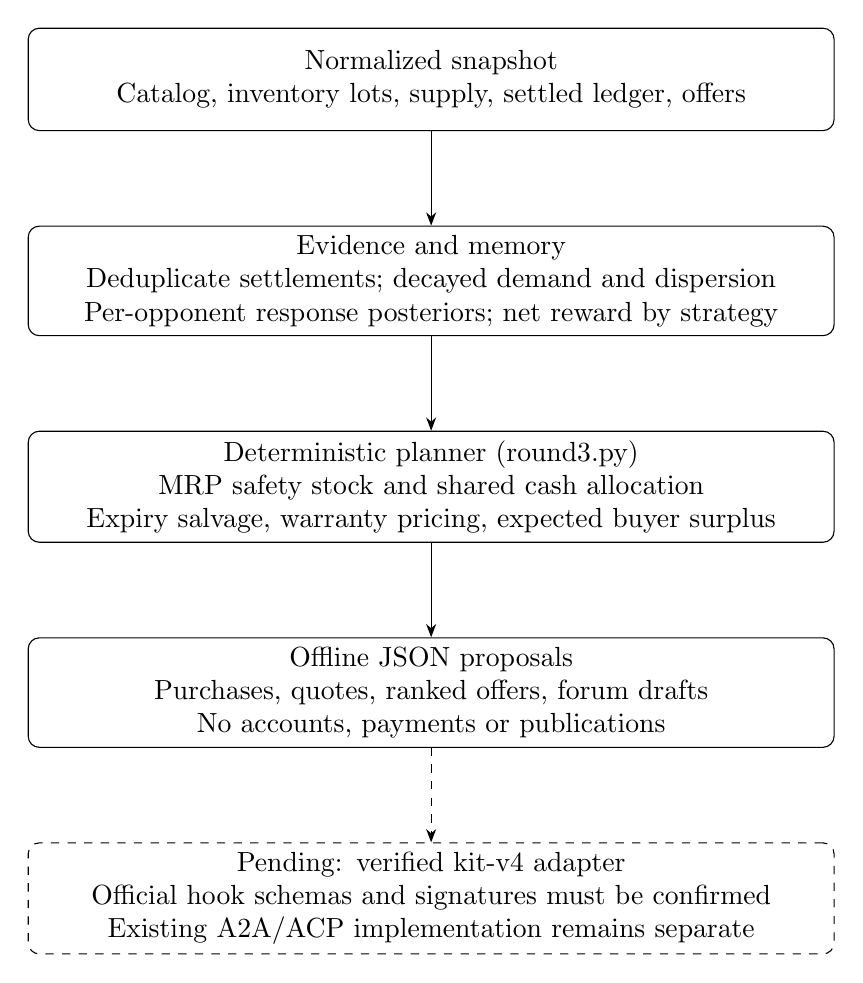
\begin{tikzpicture}[node distance=12mm,box/.style={draw,rounded corners,text width=10cm,align=center,minimum height=13mm},>=Stealth]
\node[box] (input) {Normalized snapshot\\Catalog, inventory lots, supply, settled ledger, offers};
\node[box,below=of input] (memory) {Evidence and memory\\Deduplicate settlements; decayed demand and dispersion\\Per-opponent response posteriors; net reward by strategy};
\node[box,below=of memory] (plan) {Deterministic planner (round3.py)\\MRP safety stock and shared cash allocation\\Expiry salvage, warranty pricing, expected buyer surplus};
\node[box,below=of plan] (output) {Offline JSON proposals\\Purchases, quotes, ranked offers, forum drafts\\No accounts, payments or publications};
\node[box,dashed,below=of output] (adapter) {Pending: verified kit-v4 adapter\\Official hook schemas and signatures must be confirmed\\Existing A2A/ACP implementation remains separate};
\draw[->] (input)--(memory);
\draw[->] (memory)--(plan);
\draw[->] (plan)--(output);
\draw[->,dashed] (output)--(adapter);
\end{tikzpicture}
\end{center}
This figure describes the current implementation. No live Round-3 results are
claimed. The existing model-generated week-08 policy has not been retrained or
connected to the new planner. Risk and quality inputs are estimates supplied in
the snapshot; they are not privileged observations of hidden market state.
\end{document}
